\chapter{อณูชีววิทยา เมตาเจโนมิกส์ และชีวสารสนเทศศาสตร์ทางการเกษตร}
\label{ch:metagenomics}

\begin{keyconcept}[แนวคิดสำคัญของบทที่ 9]
มากกว่าร้อยละ 99 ของจุลินทรีย์ในดินและสิ่งแวดล้อมจัดเป็นกลุ่มที่ไม่สามารถเพาะเลี้ยงได้ในห้องปฏิบัติการทั่วไป (Unculturable Microorganisms) ความก้าวหน้าของการหาลำดับเบสยุคใหม่ (Next-Generation Sequencing: NGS) และชีวสารสนเทศศาสตร์ (Bioinformatics) ได้เปิดประตูสู่ยุค \textbf{เมตาเจโนมิกส์ (Metagenomics)\index{เมตาเจโนมิกส์ (Metagenomics)}} ซึ่งเป็นการศึกษาสารพันธุกรรมทั้งหมดของชุมชนจุลินทรีย์จากตัวอย่างดินโดยตรง การเปลี่ยนผ่านจากหน่วย OTU แบบเดิมสู่ \textbf{Amplicon Sequence Variants (ASVs)\index{Amplicon Sequence Variants (ASVs)}} ด้วยไปป์ไลน์ DADA2\index{DADA2 pipeline} และ QIIME2\index{QIIME 2} ช่วยให้นักวิทยาศาสตร์สามารถประเมินดัชนีความหลากหลาย Alpha/Beta Diversity\index{ความหลากหลายของสายพันธุ์ (Alpha Diversity)}\index{Beta Diversity} และสร้างแบบจำลองเครือข่ายสหสัมพันธ์ (Co-occurrence Networks)\index{เครือข่ายสังคมจุลินทรีย์ (Co-occurrence Networks)} เพื่อนำไปสู่การออกแบบ \textbf{กลุ่มจุลินทรีย์สังเคราะห์ (Synthetic Communities: SynComs)\index{กลุ่มจุลินทรีย์สังเคราะห์ (SynComs)}} ที่มีความสามารถจำเพาะในการส่งเสริมผลผลิตและระงับโรคพืชได้อย่างมีเสถียรภาพ
\end{keyconcept}

\begin{figure}[ht]
    \centering
    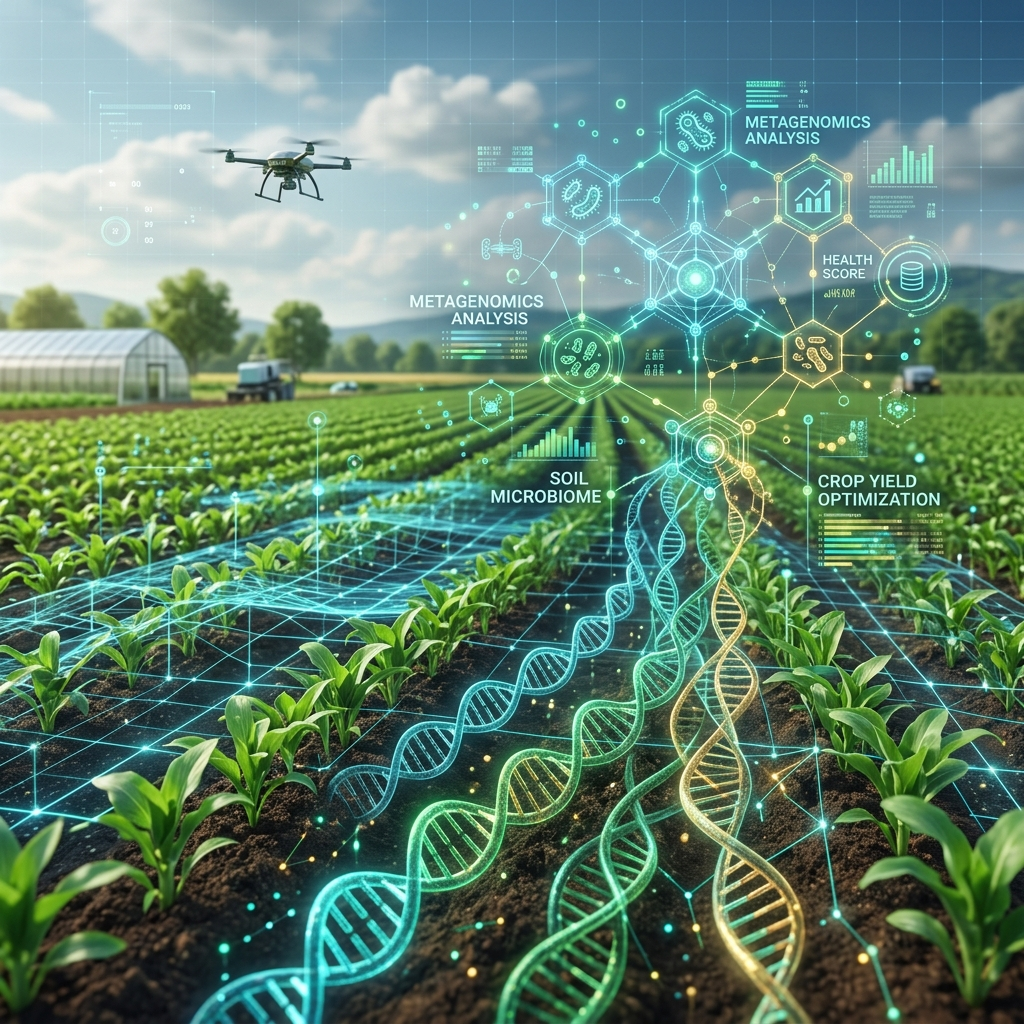
\includegraphics[width=0.85\textwidth]{assets/ch09_metagenomics_ai.png}
    \caption{การจำลอง 3D แสดงขั้นตอนการสกัด DNA จากดินไรโซสเฟียร์ การถอดรหัสพันธุกรรมเมตาเจโนมิกส์ และการวิเคราะห์เครือข่ายสังคมจุลินทรีย์ดิน (Microbial Network) ด้วยซอฟต์แวร์ชีวสารสนเทศศาสตร์ เพื่อคัดเลือกสายพันธุ์หลัก (Hub taxa) สู่การสร้างกลุ่มจุลินทรีย์สังเคราะห์}
    \label{fig:ch09_metagenomics_ai}
\end{figure}

\section*{วัตถุประสงค์การเรียนรู้ประจำบท}
เมื่อศึกษาบทเรียนนี้จบแล้ว นักศึกษาสามารถ:
\begin{enumerate}
    \item เปรียบเทียบข้อแตกต่างเชิงเทคนิคระหว่าง 16S/ITS Amplicon Sequencing และ Whole Metagenome Shotgun (WGS)
    \item วิเคราะห์ขั้นตอนการทำงานของไปป์ไลน์ชีวสารสนเทศศาสตร์มาตรฐาน (FastQC $\rightarrow$ Trimmomatic $\rightarrow$ DADA2 $\rightarrow$ QIIME2)
    \item คำนวณและแปลผลดัชนีความหลากหลายระดับท้องถิ่น (Alpha Diversity: Shannon, Simpson, Chao1) และความแตกต่างระหว่างกลุ่ม (Beta Diversity: Bray-Curtis, UniFrac)
    \item อธิบายหลักการวิเคราะห์เครือข่ายสังคมจุลินทรีย์ (Co-occurrence Networks) และการระบุชนิดพันธุ์ศูนย์กลาง (Keystone Hub Taxa)
    \item ออกแบบสูตรกลุ่มจุลินทรีย์สังเคราะห์ (SynComs) จากการบูรณาการข้อมูลเมตาเจโนมิกส์เพื่อแก้ปัญหาดินเหนียวแน่นและโรคระบาดในแปลงเกษตร
\end{enumerate}

\section{เทคโนโลยีถอดรหัสพันธุกรรมเมตาเจโนมิกส์ในดินเกษตร}

การศึกษาจุลินทรีย์ดินในยุคปัจจุบันแบ่งออกเป็น 2 แนวทางหลักตามระดับความลึกของข้อมูล:

\subsection{1. การจัดทำโพรไฟล์ยีนเครื่องหมาย (Amplicon Targeted Sequencing)}
เป็นการเพิ่มปริมาณยีนเป้าหมายที่มีบริเวณอนุรักษ์ (Conserved regions) สลับกับบริเวณที่มีความผันแปรสูง (Hypervariable regions) ด้วยเทคนิค PCR ก่อนส่งตรวจ NGS:
\begin{itemize}
    \item \textbf{แบคทีเรียและอาร์เคีย:} นิยมใช้ยีน \textbf{16S rRNA\index{16S rRNA gene sequencing}} โดยเฉพาะบริเวณผันแปร $V3-V4$ หรือ $V4$ ขนาดประมาณ 250--460 คู่เบส ซึ่งมีฐานข้อมูลอ้างอิงระดับโลก เช่น SILVA และ Greengenes
    \item \textbf{เชื้อราในดิน:} นิยมใช้บริเวณ \textbf{Internal Transcribed Spacer (ITS)\index{Internal Transcribed Spacer (ITS)}} ได้แก่ ITS1 หรือ ITS2 ซึ่งแทรกอยู่ระหว่างยีน 18S, 5.8S, และ 28S rRNA โดยเทียบกับฐานข้อมูล UNITE
\end{itemize}

\subsection{2. ช็อตกันเมตาเจโนมิกส์ทั้งชุมชน (Whole Metagenome Shotgun: WGS)}
เป็นการสกัด DNA ทั้งหมดในตัวอย่างดิน ตัดชิ้นส่วนให้สั้นลง แล้วหาลำดับเบสพร้อมกันทั้งหมดโดยไม่ผ่านการเพิ่มขยายยีนด้วย PCR (PCR-free):\index{Whole Metagenome Shotgun (WGS)}
\begin{itemize}
    \item ให้ข้อมูลทั้งโครงสร้างชนิดพันธุ์ (Taxonomic profiling) และข้อมูลหน้าที่ของยีนทั้งระบบ (Functional profiling) เช่น ยีนสร้างเอนไซม์ไนโตรจีเนส (\textit{nifH}), ยีนละลายฟอสเฟต (\textit{phoD}), หรือยีนสร้างยาปฏิชีวนะ (NRPS/PKS)
    \item สามารถนำชิ้นส่วนเบสมาต่อกัน (De novo assembly) จนได้จีโนมจุลินทรีย์ที่สมบูรณ์จากสิ่งแวดล้อม เรียกว่า **Metagenome-Assembled Genomes (MAGs)** แม้จะไม่เคยเพาะเลี้ยงเชื้อนั้นได้มาก่อน
\end{itemize}

\section{เวิร์กโฟลว์ชีวสารสนเทศศาสตร์: จากข้อมูลดิบสู่ ASVs}

\begin{figure}[ht]
\centering
\begin{tikzpicture}[node distance=1.5cm, auto,
    block/.style={rectangle, draw, fill=blue!10, text width=10.0cm, rounded corners, minimum height=0.9cm, align=left},
    arrow/.style={thick, ->, >=stealth}]
    
    \node [block] (step1) {\textbf{1. Raw FastQ Reads:} ตรวจสอบคุณภาพด้วย FastQC และ MultiQC};
    \node [block, below of=step1] (step2) {\textbf{2. Preprocessing:} ตัดไพรเมอร์ด้วย Cutadapt และกรองเบสคุณภาพต่ำด้วย Trimmomatic};
    \node [block, below of=step2] (step3) {\textbf{3. Denoising (DADA2):} สร้างโมเดลความคลาดเคลื่อนเบส แยกความแปรผันทางชีววิทยาออกจาก Noise ได้ตาราง Amplicon Sequence Variants (ASVs) ที่ความละเอียดระดับ 1 นิวคลีโอไทด์};
    \node [block, below of=step3] (step4) {\textbf{4. Chimera Removal:} ตรวจจับและกำจัดสายผสมไคเมรา};
    \node [block, below of=step4] (step5) {\textbf{5. QIIME2 Pipeline:} ระบุอนุกรมวิธานด้วย Naive Bayes Classifier เทียบฐานข้อมูล SILVA/UNITE และสร้างแผนภูมิต้นไม้ไฟโลเจเนติก};
    
    \draw [arrow] (step1) -- (step2);
    \draw [arrow] (step2) -- (step3);
    \draw [arrow] (step3) -- (step4);
    \draw [arrow] (step4) -- (step5);
\end{tikzpicture}
\caption{เวิร์กโฟลว์การประมวลผลข้อมูลชีวสารสนเทศศาสตร์เมตาเจโนมิกส์ด้วย DADA2 และ QIIME2}
\label{fig:bioinfo_pipeline}
\end{figure}

ในอดีต นักชีวสารสนเทศศาสตร์นิยมจัดกลุ่มลำดับเบสที่มีความเหมือนกัน $97\%$ ให้เป็นหนึ่งหน่วย Operational Taxonomic Unit (OTU) แต่วิธีนี้มีความคลาดเคลื่อนสูงและซ่อนความแตกต่างระดับสายพันธุ์ ในปัจจุบัน วงการวิจัยสากลได้เปลี่ยนมาใช้ **Amplicon Sequence Variants (ASVs)** ซึ่งพัฒนาโดย Callahan และคณะ (2016) \cite{callahan2016dada2} ร่วมกับแพลตฟอร์ม QIIME2 \cite{bolyen2019qiime2}:
\begin{itemize}
    \item อัลกอริทึม DADA2 ใช้แบบจำลองความน่าจะเป็นตามสถิติของเครื่องซีเควนเซอร์ เพื่อตัดสัญญาณรบกวน (Denoising) ทำให้สามารถแยกความแตกต่างของสายพันธุ์ที่มีลำดับเบสต่างกันเพียงตัวเดียว ($1\text{ bp difference}$) ได้อย่างแม่นยำ
    \item ข้อมูล ASVs เป็นค่าสัมบูรณ์ที่มีความเที่ยงตรงสูง สามารถนำตาราง ASVs จากการทดลองต่างสถานที่หรือต่างช่วงเวลามาเปรียบเทียบข้ามชุดข้อมูลกันได้โดยตรง
\end{itemize}

\section{ดัชนีชี้วัดความหลากหลายทางนิเวศวิทยาของจุลินทรีย์ดิน}

\subsection{1. ดัชนีความหลากหลายภายในแหล่งอาศัย (Alpha Diversity)}
ประเมินความหลากหลายและความสม่ำเสมอของประชากรจุลินทรีย์ภายในตัวอย่างดินหนึ่งๆ:\index{ความหลากหลายของสายพันธุ์ (Alpha Diversity)}
\begin{itemize}
    \item \textbf{Richness ($S$):} จำนวนชนิดหรือจำนวน ASVs ทั้งหมดที่ตรวจพบ
    \item \textbf{Shannon Diversity Index ($H'$):\index{Shannon Diversity Index ($H'$)}} วัดทั้งความหลากหลายของชนิดพันธุ์และความสม่ำเสมอ (Evenness) ในการกระจายตัว:
    \begin{equation}
    H' = - \sum_{i=1}^{S} p_i \ln(p_i)
    \end{equation}
    เมื่อ $p_i = n_i / N$ คือสัดส่วนความหนาแน่นสัมพัทธ์ของ ASV ลำดับที่ $i$
    \item \textbf{Simpson's Diversity Index ($D$ และ $1/D$):\index{Simpson's Diversity Index}} วัดความน่าจะเป็นที่เมื่อสุ่มเลือกจุลินทรีย์ 2 ตัวขึ้นมาแล้วจะพบว่าเป็นชนิดเดียวกัน:
    \begin{equation}
    D = \sum_{i=1}^{S} p_i^2 \quad \implies \quad \text{Inverse Simpson} = \frac{1}{D} = \frac{1}{\sum p_i^2}
    \end{equation}
    \item \textbf{Chao1 Estimator:\index{Chao1 Estimator}} ตัวประมาณการความหลากหลายที่แท้จริง โดยคำนึงถึงชนิดพันธุ์ที่พบน้อย (Rare taxa) ทั้งที่พบเพียงครั้งเดียว ($F_1$: Singletons) และพบสองครั้ง ($F_2$: Doubletons):
    \begin{equation}
    S_{\text{Chao1}} = S_{\text{obs}} + \frac{F_1 (F_1 - 1)}{2 (F_2 + 1)}
    \end{equation}
\end{itemize}

\subsection{2. ดัชนีความแตกต่างระหว่างแหล่งอาศัย (Beta Diversity)}
ประเมินความแตกต่างของโครงสร้างชุมชนจุลินทรีย์ระหว่างตัวอย่างดินต่างกรรมวิธี (เช่น ดินเกษตรอินทรีย์ vs ดินเกษตรเคมี):\index{Beta Diversity}
\begin{itemize}
    \item \textbf{Bray-Curtis Dissimilarity ($BC_{jk}$):\index{Bray-Curtis Dissimilarity}} คำนึงถึงความหนาแน่นสัมพัทธ์ของแต่ละชนิด:
    \begin{equation}
    BC_{jk} = \frac{\sum_{i=1}^{S} |n_{ij} - n_{ik}|}{\sum_{i=1}^{S} (n_{ij} + n_{ik})} = 1 - \frac{2 C_{jk}}{S_j + S_k}
    \end{equation}
    ค่า $BC = 0$ หมายถึงชุมชนจุลินทรีย์เหมือนกันทุกประการ และ $BC = 1$ หมายถึงไม่มีสปีชีส์ใดร่วมกันเลย
    \item \textbf{UniFrac Distance (Weighted / Unweighted):} ดัชนีที่บูรณาการความสัมพันธ์ทางสายวิวัฒนาการ (Phylogenetic distance) บนต้นไม้สายสัมพันธ์เข้าด้วยกัน
\end{itemize}

\section{เครือข่ายสังคมจุลินทรีย์และกลุ่มจุลินทรีย์สังเคราะห์ (SynComs)}

ในสภาพแวดล้อมดิน จุลินทรีย์ไม่ได้อาศัยอยู่อย่างโดดเดี่ยว แต่เชื่อมโยงกันเป็นเครือข่ายปฏิสัมพันธ์ (Co-occurrence Network):\index{เครือข่ายสังคมจุลินทรีย์ (Co-occurrence Networks)}

\subsection{1. การวิเคราะห์โครงสร้างเครือข่าย (Network Topologies)}
การใช้สถิติสหสัมพันธ์แบบ Spearman หรือ Sparse Correlations for Compositional Data (SparCC) ช่วยระบุความสัมพันธ์:
\begin{itemize}
    \item \textbf{Positive Edge (ขอบบวก):} แสดงถึงการเกื้อกูลกัน การใช้อาหารร่วมกัน (Syntrophy) หรือการอยู่อาศัยในถิ่นอาศัยเดียวกัน
    \item \textbf{Negative Edge (ขอบลบ):} แสดงถึงการแก่งแย่งแข่งขันสารอาหาร (Competition) หรือการสร้างสารปฏิชีวนะยับยั้งกัน (Amensalism)
    \item \textbf{Keystone Hub Taxa (ชนิดพันธุ์แกนหลัก):\index{Keystone Hub Taxa}} จุลินทรีย์ที่มีค่า Degree Centrality และ Closeness Centrality สูงมาก หากกำจัดจุลินทรีย์แกนหลักเหล่านี้ออก เครือข่ายไมโครไบโอมในดินจะพังทลายลงทันที
\end{itemize}

\subsection{2. การออกแบบกลุ่มจุลินทรีย์สังเคราะห์ (Synthetic Communities: SynComs)}
Vorholt และคณะ (2017) \cite{vorholt2017syncom} ได้วางกรอบแนวคิดการสร้าง \textbf{SynComs\index{กลุ่มจุลินทรีย์สังเคราะห์ (SynComs)}} ซึ่งเป็นการคัดเลือกจุลินทรีย์ที่เพาะเลี้ยงได้จำนวนหนึ่ง (ปกติ 5--20 สายพันธุ์) ที่มีหน้าที่ทางชีวเคมีเกื้อหนุนกันตามข้อมูลเมตาเจโนมิกส์:
\begin{enumerate}
    \item สายพันธุ์ที่ 1: ตรึงไนโตรเจน (\organism{Azospirillum brasilense})
    \item สายพันธุ์ที่ 2: ละลายฟอสเฟต (\organism{Bacillus velezensis})
    \item สายพันธุ์ที่ 3: สังเคราะห์สารไซเดอโรฟอร์จับเหล็ก (\organism{Pseudomonas putida})
    \item สายพันธุ์ที่ 4: ผลิตเอนไซม์ ACC Deaminase ลดความเครียดพืช
    \item สายพันธุ์ที่ 5: ป้องกันเชื้อราก่อโรคด้วยสารไลโปเปปไทด์
\end{enumerate}
การรวมกลุ่มแบบ SynComs ช่วยแก้ปัญหาความล้มเหลวของการใช้หัวเชื้อเดี่ยว (Single-strain inoculant) ในแปลงเกษตรจริงได้อย่างยั่งยืน

\begin{application}[กรณีศึกษางานวิจัย RBRU: การวิเคราะห์ 16S Amplicon Metagenomics ในสวนทุเรียน จ.จันทบุรี]
จากงานวิจัยของ Jantamalee \& Thassana (2025) \cite{jantamalee_2025} ณ มหาวิทยาลัยราชภัฏรำไพพรรณี\index{งานวิจัย RBRU!16S Metagenomics สวนทุเรียน} ได้ดำเนินการสกัด Soil DNA และถอดรหัสลำดับเบสบริเวณยีน 16S rRNA (V3--V4 region) ด้วยเทคโนโลยี Illumina NovaSeq 6000 ในดินไรโซสเฟียร์สวนทุเรียนพันธุ์หมอนทอง 2 กลุ่มจัดการ ได้แก่ แปลงเกษตรอินทรีย์ชีวภาพ (อ.เขาคิชฌกูฏ) และแปลงเกษตรเคมีเข้มข้น (อ.ท่าใหม่):
\begin{itemize}
    \item \textbf{Alpha Diversity:} แปลงเกษตรอินทรีย์มีค่า Shannon Index สูงถึง $H' = 4.86 \pm 0.14$ และ Chao1 $= 1,420$ เทียบกับแปลงเกษตรเคมีที่พบเพียง $H' = 3.18 \pm 0.22$ และ Chao1 $= 780$ แสดงถึงการสูญเสียความหลากหลายอย่างรุนแรงจากการใช้สารเคมีต่อเนื่อง
    \item \textbf{Taxonomic Profiling:} ดินอินทรีย์อุดมไปด้วยไฟลัม \textit{Firmicutes} (สกุล \organism{Bacillus}) และ \textit{Actinobacteria} (สกุล \organism{Streptomyces}) ในสัดส่วนรวมกันมากกว่าร้อยละ 45 ขณะที่แปลงเคมีมีสัดส่วนของ \textit{Proteobacteria} ฉวยโอกาสเพิ่มขึ้น
    \item \textbf{Co-occurrence Network:} การวิเคราะห์เครือข่ายระบุว่า \organism{Bacillus velezensis} และ \organism{Bradyrhizobium} ทำหน้าที่เป็น Keystone Hub Taxa สำคัญ ซึ่งเป็นฐานข้อมูลชีวภาพในการสังเคราะห์กลุ่มจุลินทรีย์ SynComs ท้องถิ่น
\end{itemize}
\end{application}

\begin{worked}[ตัวอย่างที่ 9.1 การคำนวณ Shannon Index และ Simpson Index ของดินแปลงทุเรียน]
จากการวิเคราะห์ 16S rRNA sequencing พบสัดส่วนจำนวนนับของแบคทีเรีย 5 กลุ่มหลักในดินแปลงเกษตรอินทรีย์ที่มีสุขภาพดี:
\begin{center}
\small
\begin{tabular}{lcc}
\toprule
\textbf{กลุ่มแบคทีเรียหลัก} & \textbf{จำนวนนับ (Reads: $n_i$)} & \textbf{สัดส่วนสัมพัทธ์ ($p_i$)} \\
\midrule
1. \textit{Acidobacteria} & 3,200 & 0.32 \\
2. \textit{Actinobacteria} & 2,500 & 0.25 \\
3. \textit{Proteobacteria} & 2,100 & 0.21 \\
4. \textit{Firmicutes} & 1,400 & 0.14 \\
5. \textit{Bacteroidetes} & 800 & 0.08 \\
\midrule
\textbf{รวม ($N$)} & \textbf{10,000} & \textbf{1.00} \\
\bottomrule
\end{tabular}
\end{center}

จงคำนวณค่า Shannon Diversity Index ($H'$) และ Inverse Simpson Index ($1/D$) ของตัวอย่างดินนี้

\textbf{วิธีทำ:}
1. คำนวณค่า $p_i \ln(p_i)$ ของแต่ละกลุ่ม:
\begin{itemize}
    \item กลุ่ม 1: $0.32 \times \ln(0.32) = 0.32 \times (-1.1394) \approx -0.3646$
    \item กลุ่ม 2: $0.25 \times \ln(0.25) = 0.25 \times (-1.3863) \approx -0.3466$
    \item กลุ่ม 3: $0.21 \times \ln(0.21) = 0.21 \times (-1.5606) \approx -0.3277$
    \item กลุ่ม 4: $0.14 \times \ln(0.14) = 0.14 \times (-1.9661) \approx -0.2753$
    \item กลุ่ม 5: $0.08 \times \ln(0.08) = 0.08 \times (-2.5257) \approx -0.2021$
\end{itemize}
$$\sum p_i \ln(p_i) = -0.3646 - 0.3466 - 0.3277 - 0.2753 - 0.2021 = -1.5163$$
$$H' = -(-1.5163) \approx 1.5163$$

2. คำนวณค่า Simpson Index ($D = \sum p_i^2$):
$$D = (0.32)^2 + (0.25)^2 + (0.21)^2 + (0.14)^2 + (0.08)^2$$
$$D = 0.1024 + 0.0625 + 0.0441 + 0.0196 + 0.0064 = 0.2350$$
$$\text{Inverse Simpson } (1/D) = \frac{1}{0.2350} \approx 4.255$$

\textbf{บทวิเคราะห์ผลลัพธ์:} ค่า Shannon Index เท่ากับ 1.5163 และ Inverse Simpson เท่ากับ 4.255 บ่งชี้ว่าดินในแปลงอินทรีย์นี้มีการกระจายตัวของกลุ่มจุลินทรีย์ที่สม่ำเสมอดีมาก ไม่มีกลุ่มใดครอบงำ (Dominance) จนทำลายความหลากหลาย ซึ่งเป็นลักษณะโครงสร้างดินที่ต้านทานการเกิดโรคพืชได้ดี
\end{worked}

\begin{worked}[ตัวอย่างที่ 9.2 การคำนวณ Bray-Curtis Dissimilarity เปรียบเทียบดินสองกรรมวิธี]
นักวิจัยเก็บตัวอย่างดินจากแปลงเกษตรอินทรีย์ ($j$) และแปลงเกษตรเคมีเข้มข้น ($k$) ตรวจนับ ASVs เด่น 4 ชนิด:

\begin{center}
\small
\begin{tabular}{cccc}
\toprule
\textbf{ชนิด ASV เด่น} & \textbf{แปลงอินทรีย์ ($n_{ij}$)} & \textbf{แปลงเคมี ($n_{ik}$)} & \textbf{ผลต่าง $|n_{ij} - n_{ik}|$} \\
\midrule
ASV 1 (\textit{Rhizobium}) & 120 & 20 & 100 \\
ASV 2 (\textit{Bacillus}) & 85 & 35 & 50 \\
ASV 3 (\textit{Nitrosomonas}) & 40 & 15 & 25 \\
ASV 4 (\textit{Fusarium}) & 10 & 90 & 80 \\
\midrule
\textbf{รวม} & \textbf{255} & \textbf{160} & \textbf{255} \\
\bottomrule
\end{tabular}
\end{center}

จงคำนวณดัชนีความไม่เหมือน Bray-Curtis Dissimilarity ($BC_{jk}$) ระหว่างสองแปลงนี้

\textbf{วิธีทำ:}
$$BC_{jk} = \frac{\sum |n_{ij} - n_{ik}|}{\sum (n_{ij} + n_{ik})}$$
$$\sum |n_{ij} - n_{ik}| = 100 + 50 + 25 + 80 = 255$$
$$\sum (n_{ij} + n_{ik}) = 255 + 160 = 415$$
$$BC_{jk} = \frac{255}{415} \approx 0.6145 \text{ หรือ } 61.45\%$$

\textbf{บทวิเคราะห์ผลลัพธ์:} ค่าความไม่เหมือน Bray-Curtis เท่ากับ $61.45\%$ บ่งชี้ว่าการใช้สารเคมีส่งผลกระทบอย่างรุนแรงต่อโครงสร้างของไมโครไบโอมดิน ทำให้กลุ่มแบคทีเรียที่เป็นประโยชน์ (\textit{Rhizobium}, \textit{Bacillus}) ลดลงอย่างมีนัยสำคัญ ในขณะที่เชื้อราก่อโรคพืช (\textit{Fusarium}) เพิ่มขึ้นถึง 9 เท่า
\end{worked}

% [RESEARCH-UPDATE-2026-10]
\section{ความก้าวหน้างานวิจัยล่าสุดด้านเมตาเจโนมิกส์ทางการเกษตร}

งานวิจัยระดับแนวหน้าในปี ค.ศ. 2024–2026 โดย Clagnan และคณะ \cite{pmid39526137} ได้ผสานเทคนิคคัลเชอโรมิกส์ (Culturomics: การเพาะเลี้ยงนับร้อยสภาวะ) ร่วมกับเมตาเจโนมิกส์ความลึกสูง พบว่าการฟื้นฟูดินด้วยหัวเชื้อจุลินทรีย์สังเคราะห์ SynComs สามารถเพิ่มความอุดมสมบูรณ์ของยีนหมุนเวียนคาร์บอนและไนโตรเจนในดินที่เสื่อมโทรมได้อย่างรวดเร็ว

ในขณะเดียวกัน งานวิจัยของ Panek และคณะ \cite{pmid41800415} ได้แสดงให้เห็นว่าการวิเคราะห์เครื่องหมายเมตาเจโนมิกส์ (Metagenomic Biomarkers) สามารถใช้เป็นดัชนีเตือนภัยล่วงหน้า (Early-Warning Biomarkers) ของการพังทลายของระบบนิเวศดินก่อนที่ค่าทางเคมีกายภาพ (pH, N-P-K) จะเปลี่ยนแปลงถึง 1 ฤดูปลูก

\begin{insight}[ประเด็นวิเคราะห์เชิงวิชาการ]
เหตุใดการศึกษาความหลากหลายทางชีวภาพของแบคทีเรียในดิน จึงไม่ควรยึดติดอยู่กับลำดับเบส 16S rRNA เพียงอย่างเดียว? และข้อมูล Shotgun Metagenomics มีข้อได้เปรียบอย่างไรในการศึกษาบทบาทเชิงฟังก์ชันของยีนต้านทานยาปฏิชีวนะ (ARGs) ในดินเกษตรกรรม?
\end{insight}

\section*{สรุปประจำบท}

เทคโนโลยีเมตาเจโนมิกส์และชีวสารสนเทศศาสตร์ได้ปฏิวัติความเข้าใจเกี่ยวกับไมโครไบโอมในดินอย่างสิ้นเชิง การเปลี่ยนผ่านจากเทคนิคการเพาะเลี้ยงแบบเดิมสู่การถอดรหัสพันธุกรรมขั้นสูงทั้ง Amplicon Sequencing (ยีน 16S rRNA และบริเวณ ITS) และ Whole Metagenome Shotgun ร่วมกับไปป์ไลน์ DADA2 และ QIIME2 ช่วยให้นักวิจัยเข้าถึงความหลากหลายระดับ ASVs ได้อย่างแม่นยำ การคำนวณดัชนี Alpha Diversity (Shannon, Simpson, Chao1) และ Beta Diversity (Bray-Curtis, UniFrac) ช่วยประเมินความสมบูรณ์และเสถียรภาพของดินได้อย่างเป็นรูปธรรม ยิ่งไปกว่านั้น การทำความเข้าใจโครงสร้างเครือข่ายสังคมจุลินทรีย์และการระบุชนิดพันธุ์แกนหลัก (Hub taxa) ถือเป็นรากฐานสำคัญสู่การสร้างกลุ่มจุลินทรีย์สังเคราะห์ (SynComs) ที่ช่วยฟื้นฟูระบบนิเวศการเกษตรได้อย่างตรงจุดและยั่งยืน

\subsection*{คำถามท้ายบทและการวิเคราะห์}

\noindent \textbf{ระดับที่ 1: ความรู้และความเข้าใจเชิงทฤษฎี (Knowledge \& Comprehension)}
\begin{enumerate}
    \item เปรียบเทียบข้อดีและข้อจำกัดระหว่างการวิเคราะห์ Amplicon Sequencing (16S/ITS) กับการวิเคราะห์ Whole Metagenome Shotgun (WGS)
    \item อธิบายความแตกต่างพื้นฐานระหว่างหน่วย Operational Taxonomic Units (OTUs ที่ 97\%) กับ Amplicon Sequence Variants (ASVs) ในการวิเคราะห์ชีวสารสนเทศศาสตร์
    \item เหตุใดบริเวณยีน 16S rRNA จึงได้รับการคัดเลือกให้เป็นยีนเครื่องหมายสากลสำหรับการจัดจำแนกแบคทีเรียและอาร์เคีย?
    \item สรุปขั้นตอนการทำงานของไปป์ไลน์ชีวสารสนเทศศาสตร์มาตรฐานตั้งแต่ Raw Reads (FastQ) จนถึงการได้ตาราง ASVs ในซอฟต์แวร์ DADA2
\end{enumerate}

\noindent \textbf{ระดับที่ 2: การวิเคราะห์และการคำนวณเชิงปริมาณ (Quantitative Analysis \& Calculation)}
\begin{enumerate}[resume]
    \item อธิบายความหมายเชิงนิเวศวิทยาของดัชนี Shannon Diversity Index ($H'$) และเปรียบเทียบกับดัชนี Simpson's Index ($D$)
    \item ในการคำนวณความหลากหลาย Chao1 ตัวแปร Singletons ($F_1$) และ Doubletons ($F_2$) มีความสำคัญต่อการประมาณจำนวนชนิดพันธุ์ทั้งหมดอย่างไร?
    \item ในแปลงปลูกส้มมี ASVs ของแบคทีเรีย 3 ชนิด ด้วยจำนวนนับ $n_1 = 500$, $n_2 = 300$, และ $n_3 = 200$ จงคำนวณหาค่า Shannon Index ($H'$)
\end{enumerate}

\noindent \textbf{ระดับที่ 3: การสังเคราะห์และการแก้ปัญหาในแปลงจริง (Application \& Real-World Synthesis)}
\begin{enumerate}[resume]
    \item ดัชนี Bray-Curtis Dissimilarity ใช้วัดสิ่งใด และค่าที่ได้มีความหมายอย่างไรเมื่อเปรียบเทียบแปลงเกษตรอินทรีย์กับแปลงเกษตรเคมี?
    \item จากกรณีศึกษางานวิจัย RBRU ในสวนทุเรียน จ.จันทบุรี จงอธิบายบทบาทของ Keystone Hub Taxa ต่อเสถียรภาพของไมโครไบโอมดิน และเหตุใดการใช้สารเคมีต่อเนื่องจึงทำให้ค่า Shannon Index ลดลง?
    \item จงออกแบบขั้นตอนการคัดเลือกและทดสอบกลุ่มจุลินทรีย์สังเคราะห์ (Synthetic Communities: SynComs) จำนวน 6 สายพันธุ์ เพื่อใช้ฟื้นฟูดินเค็มและส่งเสริมการเจริญเติบโตของข้าว
\end{enumerate}
